\section{深度学习技巧总结}

为改善深度学习的效果,针对不同情况需要采取不同措施。在模型发生欠拟合和过拟合时采取的方法是不同的,结合机器学习三步骤,改善模型的选择流程如图\ref{fig:recipe_of_dl}所示。
\begin{figure}[htb]
	\centering
	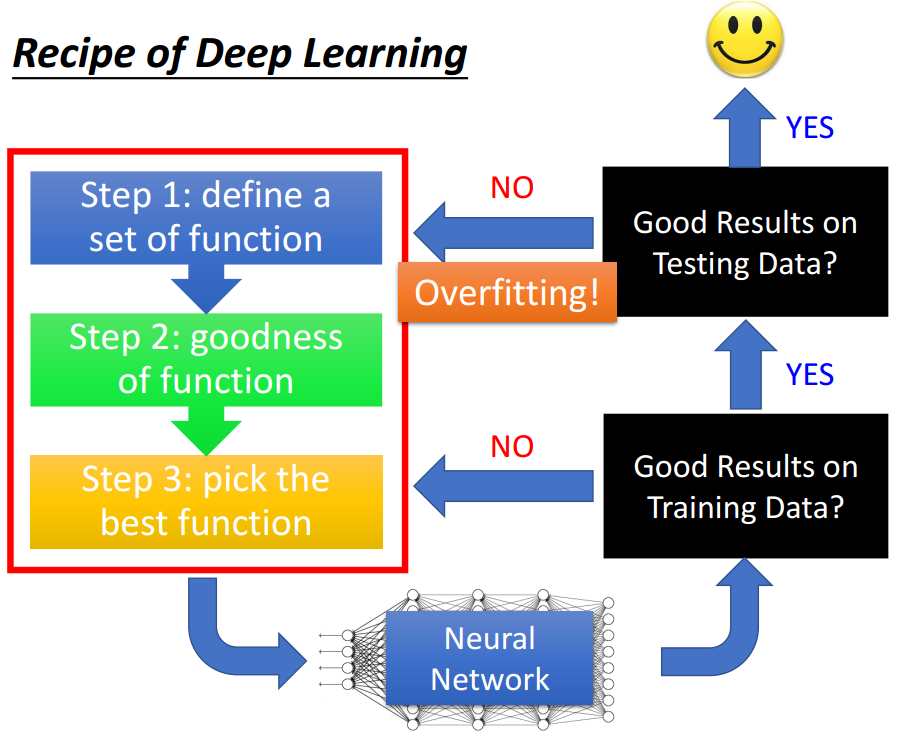
\includegraphics[scale=0.4]{pic/recipe_of_dl}
	\caption{recipe of deep learning}
	\label{fig:recipe_of_dl}
\end{figure}
因此在模型在测试集上取得比较差的结果时,必须确定是在训练阶段结果就差,还是模型发生了过拟合仅在测试集上效果较差,依次才能针对不同情况加以改善。如图\ref{fig:blame_overfitting}所示,在测试集上,更为复杂的56层网络结构的效果不如20层网络,直觉上发生了过拟合,但实际在训练阶段,56层的模型就没有训练好。因此,应该修正模型的训练过程,再在测试集上测试。
\begin{figure}[b]
	\centering
	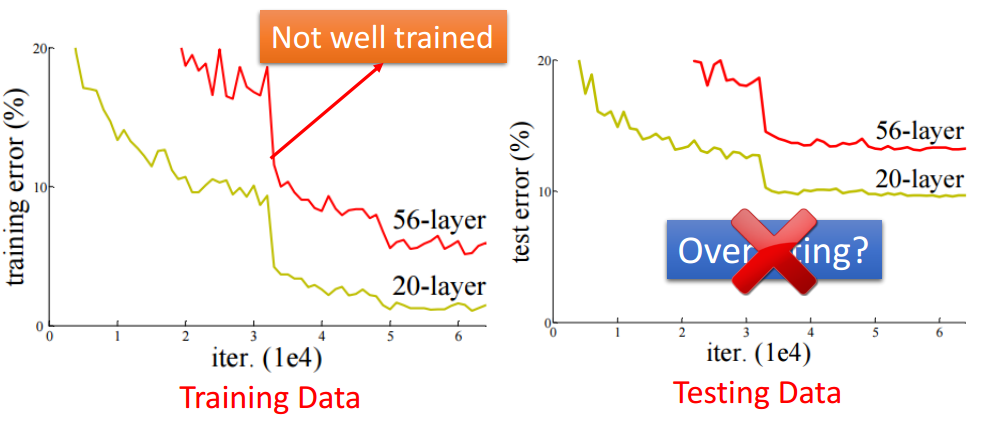
\includegraphics[scale=0.4]{pic/blame_overfitting}
	\caption{do not always blame overfitting}
	\label{fig:blame_overfitting}
\end{figure}
\begin{myquotation}{tips for overfitting and underfitting}
	
\begin{itemize}
	\item underfitting
		\subitem	选择新的激活函数
		\subitem 	自适应学习率
	\item overfitting
		\subitem	及早停止
		\subitem	正则化
		\subitem	dropout 
\end{itemize}
	
\end{myquotation}

\subsection{underfitting}

\subsubsection{梯度消失}

实际上,随着网络结构的复杂,在训练集上并不是更能够取得更优的结果,存在的主要问题就是梯度消失问题,简单的说就是,在反向传播时,靠近输入层的权重不容易得到更新,相比而言,靠近输出层的权重能够得到大的更新,如果开始阶段,权重是通过随机初始化的,那么靠近输入层的权重没有经过太大更新,还保持随机的状态,对整个网络而言,达到一个局部最优点是权重就停止更新了。

对 sigmoid 激活函数而言$\sigma ' (z) = \sigma(z)(1-\sigma(z))$,在$z=0$是取得最大值0.25。现在,如果使用标准方法来初始化网络中的权重,那么会使用一个均值为0,标准差为1的高斯分布。因此所有的权重通常会满足$|wj|<1$。从而有$\sigma'(z)w < 0.25$,前面的层上的梯度是来自后面的层上项的乘积,层数越多,靠近输入层的权重更新的就越小,这就是消失的梯度出现的本质原因。

因此,解决梯度消失问题的一个方法就是使用新的激活函数。

\subsubsection{ReLU}
\begin{equation}
\sigma(z)=\begin{cases}
0,\mathrm{if}\quad z \leq 0\\
z,\mathrm{if} \quad z > 0
\end{cases}
\end{equation}
从某种角度上看,当$z\leq 0$时,该单元没有激活,另外,在$z >0 $时,$\sigma'(z)=1$,解决了梯度消失问题。
\subsubsection{ReLU variant}
ReLU有几种变种,如leaky ReLU和parametric ReLU。区别是前者在$z\leq 0$时,取$\sigma(z)=0.01z$,后者的斜率是和梯度相关的,而非定值。

\subsubsection{maxout}
maxout 方法的主要思路是激活函数也是通过学习得到的,将网络中的单元分组,如两个一组,最终的输出结果为最大的值,思想和maxpooling 类似,示意图如图\ref{fig:maxout}所示。
\begin{figure}[htb]
	\centering
	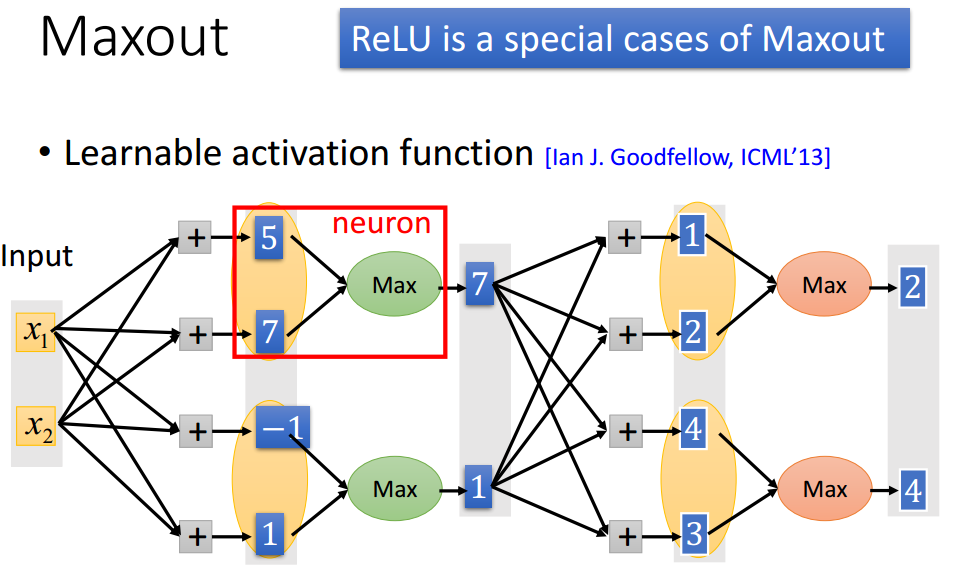
\includegraphics[scale=0.4]{pic/maxout}
	\caption{maxout 示意图}
	\label{fig:maxout}
\end{figure}

实质上,ReLU函数可以看做是 maxout 在特定情况下的特例。如图\ref{fig:relu_isa_maxout}所示:
\begin{figure}[htb]
	\centering
	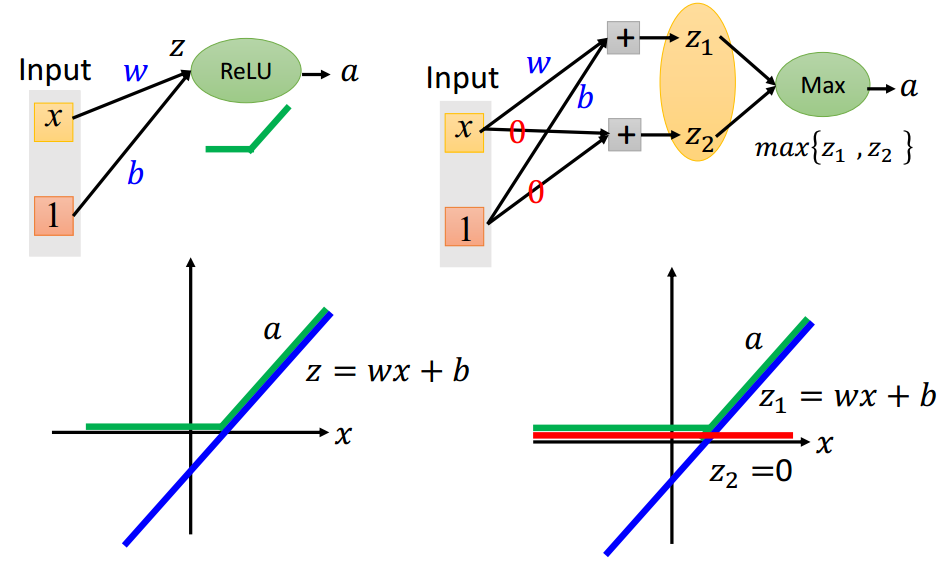
\includegraphics[scale=0.4]{pic/relu_isa_maxout}
	\caption{relu is a maxout}
	\label{fig:relu_isa_maxout}
\end{figure}

一般情况下,可以学习出不同类型的激活函数,激活函数的线性形状与权值有关,如图\ref{fig:learnable_activation}所示:

\begin{figure}[htb]
	\centering
	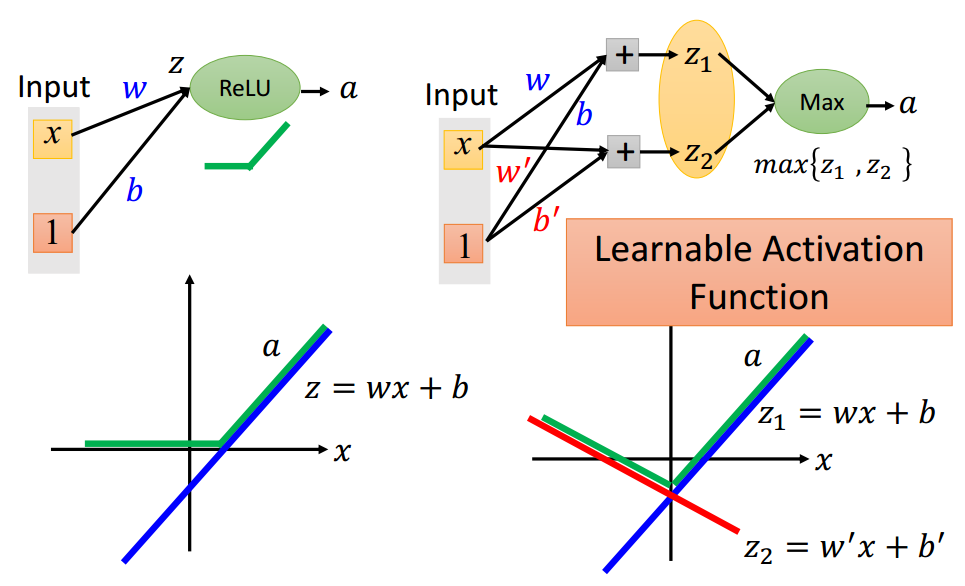
\includegraphics[scale=0.4]{pic/learnable_activation}
	\caption{learnable activation}
	\label{fig:learnable_activation}
\end{figure}

激活函数的线性分段数与单元的分组情况有关,如两段和三段的情况如图\ref{fig:pieces_of_activation}所示:
\begin{figure}[htb]
	\centering
	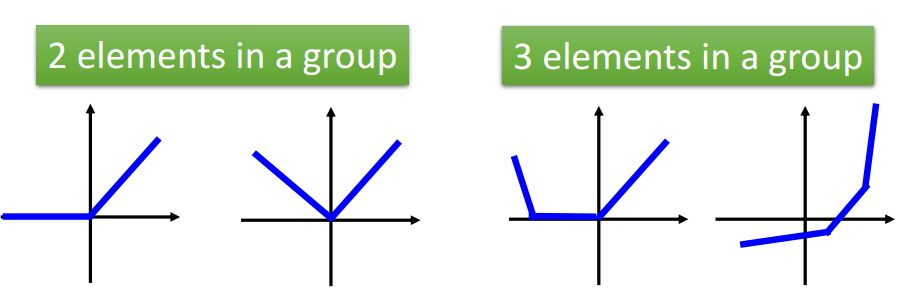
\includegraphics[scale=0.4]{pic/pieces_of_activation}
	\caption{pieces of activation}
	\label{fig:pieces_of_activation}
\end{figure}

实质上,maxout 方法也如同ReLU 函数,每次仅有有限的单元被激活,也只有被激活的单元权重会被更新,但不总是仅有某些单元一直失活,随着输入数据的不同,不同的单元会失活。

\subsubsection{自适应学习率}
adagrad:使用所有迭代的一阶导数来近似二阶导数
\[
w ^ { t + 1 } \leftarrow w ^ { t } - \frac { \eta } { \sqrt { \sum _ { i = 0 } ^ { t } \left( g ^ { i } \right) ^ { 2 } } } g ^ { t }
\]

RMSprop:
\begin{align}
w ^ { 1 } \leftarrow w ^ { 0 } - \frac { \eta } { \sigma ^ { 0 } } g ^ { 0 } \qquad & \sigma ^ { 0 } = g ^ { 0 }\\
w ^ { 2 } \leftarrow w ^ { 1 } - \frac { \eta } { \sigma ^ { 1 } } g ^ { 1 } \qquad & \sigma ^ { 1 } = \sqrt { \alpha \left( \sigma ^ { 0 } \right) ^ { 2 } + ( 1 - \alpha ) \left( g ^ { 1 } \right) ^ { 2 } }\\
w ^ { t + 1 } \leftarrow w ^ { t } - \frac { \eta } { \sigma ^ { t } } g ^ { t } \qquad & \sigma ^ { t } = \sqrt { \alpha \left( \sigma ^ { t - 1 } \right) ^ { 2 } + ( 1 - \alpha ) \left( g ^ { t } \right) ^ { 2 } }
\end{align}

未解决在局部最优点、saddle point、plateau等导数为零或近似于零的地方权重停止更新,从物理领域进入了动量的概念,解决此问题。

Momentum:
与经典的梯度下降法中权重的更新方式,momentum中也每一步前的权重更新的方向考虑在内,实际上是以前所有的梯度都考虑在内,只不过越远的权重的比例越小。对比如图\ref{fig:gd_vs_monentum}所示。
\begin{figure}[htb]
	\centering
	
	{\subcaptionbox{gradient decent}{%
			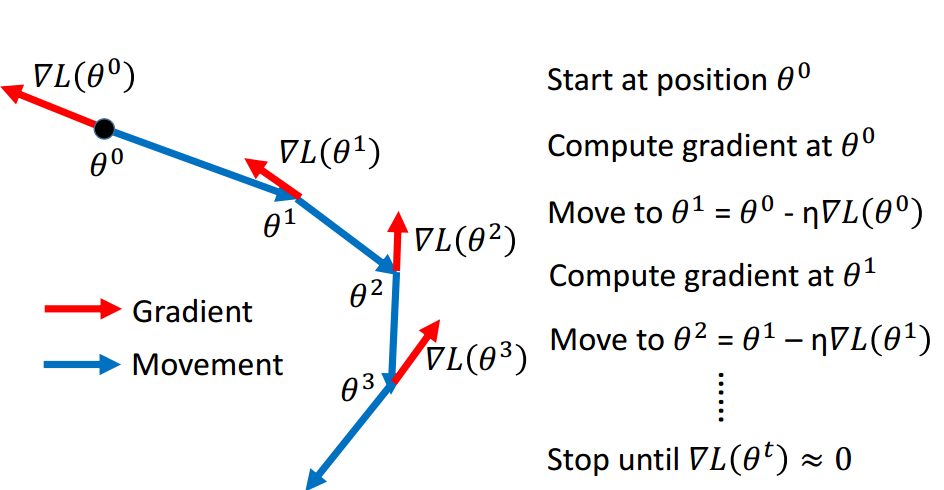
\includegraphics[scale=0.4]{pic/gd_plot}}\quad
		\subcaptionbox{momentum}{%
			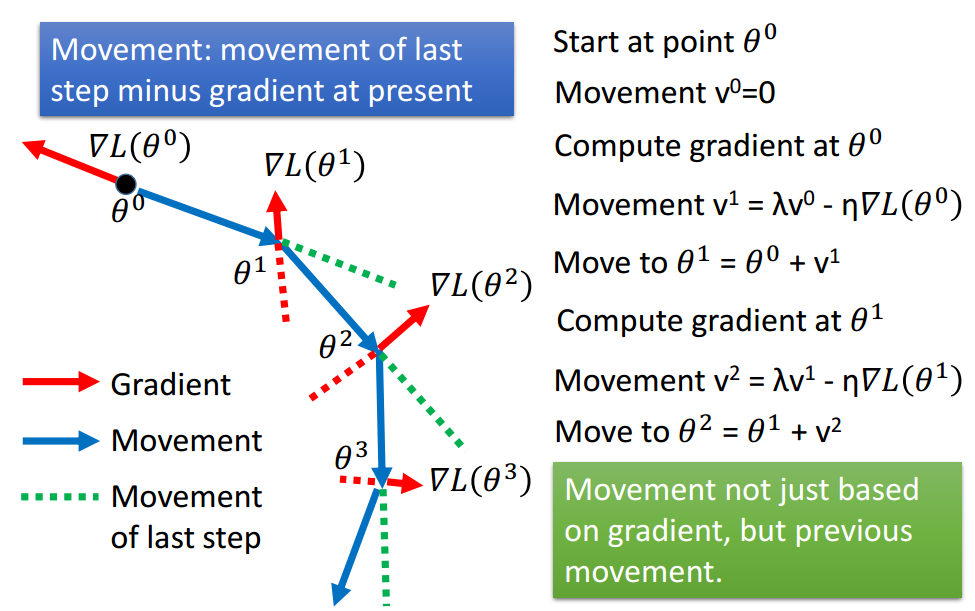
\includegraphics[scale=0.4]{pic/momentum_plot}}
	}
	\caption{经典梯度权重更新与momentum 方法}
	\label{fig:gd_vs_monentum}
\end{figure}

momentum 中每一步权重增量公式如图\ref{fig:momentum_weight}所示。
\begin{figure}[htb]
	\centering
	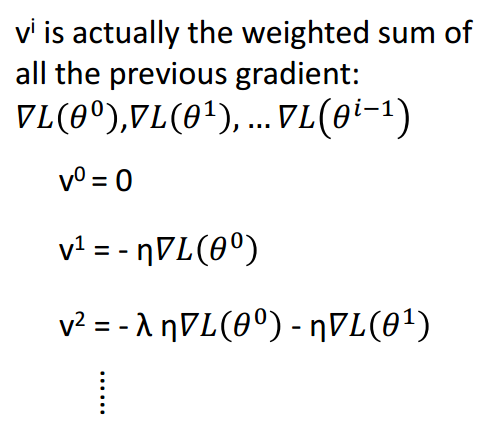
\includegraphics[scale=0.4]{pic/momentum_weight}
	\caption{momentum weight increment}
	\label{fig:momentum_weight}
\end{figure}

Adam:将adagrad与RMSprop结合,具体如图\ref{fig:adam}。

\begin{figure}[htb]
	\centering
	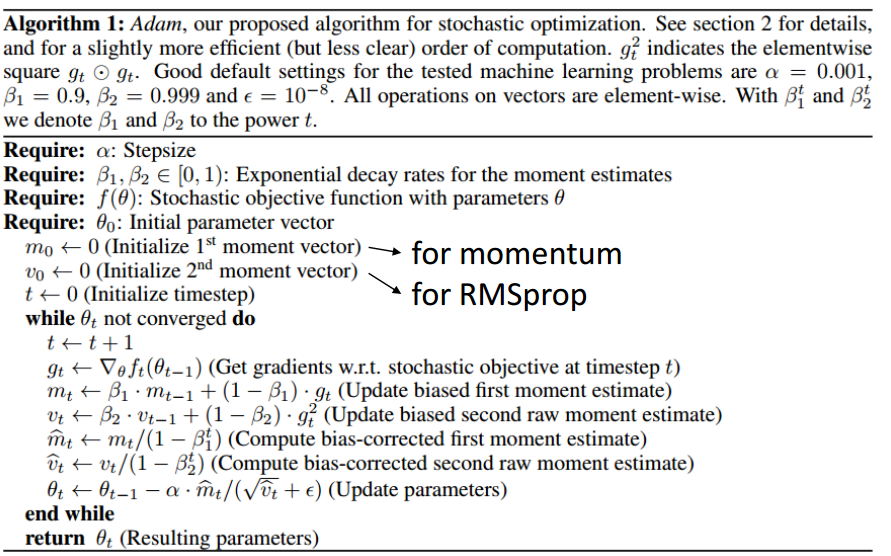
\includegraphics[scale=0.6]{pic/adam}
	\caption{adam 方法}
	\label{fig:adam}
\end{figure}

\subsection{overfitting}

\subsubsection{及早停止}
顾名思义,过拟合时在测试集上的正确率不减反增,所以选择合适的epoch停止网络训练,当然,这里的测试集指的是验证集。
\subsubsection{正则化}

\subsubsection{dropout}